\section{Validation}
\label{sec:evaluation}
In this section, we demonstrate by example that our algorithm satisfies the properties we set up as the goodness-of-split criteria for good small multiple displays.


\subsection{Visually Rich}
Our first criterion is to prefer small multiple displays that have visually salient patterns. Our algorithm achieves this through its use of the input cognostic  in measuring the presence and extent of a visual pattern in component plots of a small multiple display. 
We demonstrate this using the visual pattern of striation captured by a scagnostic~\cite{Wilkinson2005}. Consider the bivariate relationship between linolenic and linoleic in Figure~\ref{fig:vrich_all} from the olive oils dataset~\cite{Forina1983}, which represents eight chemical measurements on different specimens of olive oil produced in various regions in Italy. There appears to be visually striking clumps and striation patterns overlaid. An analyst might wonder whether these patterns can be isolated and explained by any of the other variables in the dataset.

\begin{figure}
 \centering 
	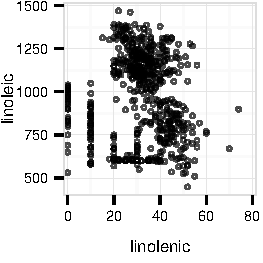
\includegraphics[width=1.75in]{images/linolenic-linoleic.pdf}
	  \caption{User-selected bivariate relationship of two chemicals in the Olive oils dataset. }
	 \label{fig:vrich_all}
\end{figure}

\begin{figure}
	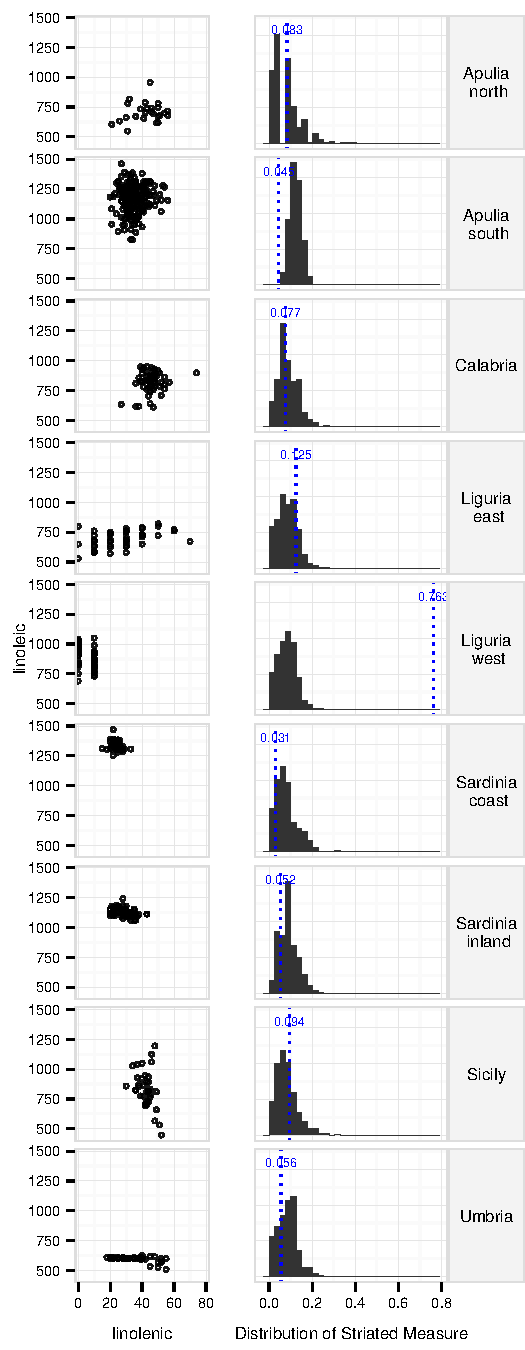
\includegraphics[width=3.25in]{images/15_729035813077-region.pdf}
	  \caption{The highest ranked small multiple on the Striation scagnostic pulls apart the striated patterns from the original bivariate relationship. }
	 \label{fig:vrich_sm}
\end{figure}

(DO WE NEED MORE DETAIL HERE?)
Our approach ranks the ``Region" variable as the best partitioning variable for isolating a striated pattern. Figure~\ref{fig:vrich_sm} reveals the clean isolation of the striation pattern for olive oils from the Liguria region and the distinctive measurement structures of linoleic values for the Umbria region. This small multiple explains the visually rich patterns seen in the original bivariate plot. 


\subsection{Informative}
We want small multiple displays that reveal unusual structure when compared to that seen in the original view. Such a partitioning of the data adds to the user's understanding of the dataset. Different visual patterns in component plots function as an indicator of the partitioning variable's explanatory power and its independence relative to the response variables being examined. 
Our algorithm finds informative small multiples by its use of permutation tests to find ones that are significantly different from ones created by randomly sampling the original view.

\begin{figure}
 \centering 
	 \begin{subfigure}{1.5in}
		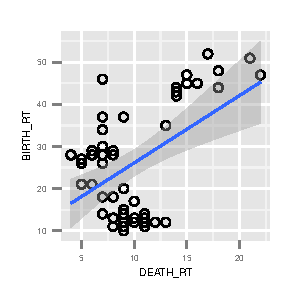
\includegraphics[width=1.5in]{images/DEATH_RT-BIRTH_RT.pdf}
		  \caption{}
		 \label{fig:informative_all}
	\end{subfigure}
	\begin{subfigure}{3in}
		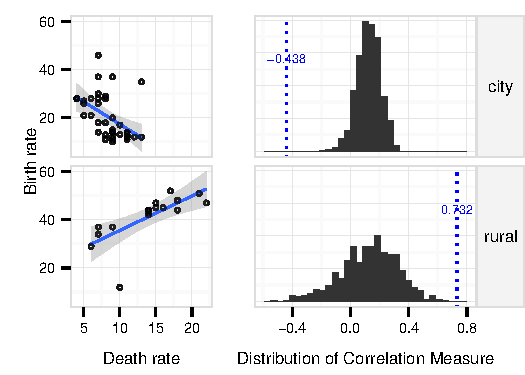
\includegraphics[width=3in]{images/7_05653068514253-URBAN.pdf}
		 \label{fig:informative_sm}
		  \caption{}
	 \end{subfigure}
	\begin{subfigure}{3in}
		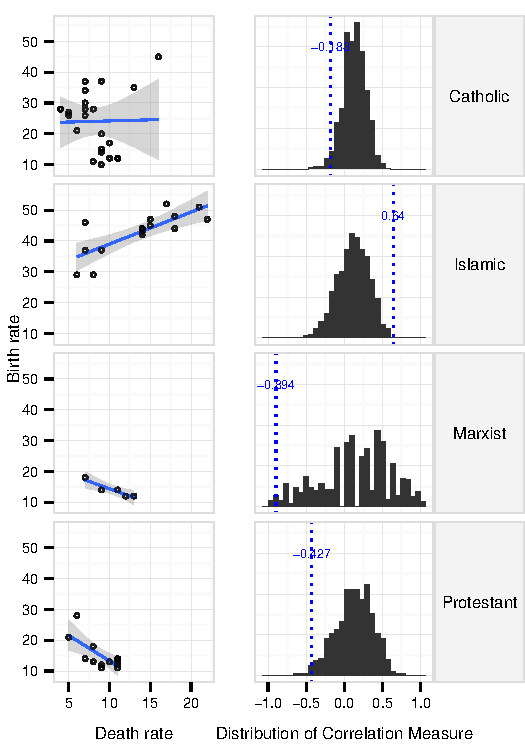
\includegraphics[width=3in]{images/2_56911395752061-LEADER.pdf}
		  \caption{}
		 \label{fig:informative_sm_big}
	 \end{subfigure}
	  \caption{(a) User-selected relationship between birth and death rates for countries around the world. (b) The highest ranked small multiple display shows partitions that reveal strong opposite trends that were not seen in the original view. (c) The lowest ranked small multiple display that reveals interesting correlations but is not parsimonious.}
\end{figure}

An illustration of an informative view involves the use of the Monotonic scagnostic~\cite{Wilkinson2005} and the Ourworld dataset of UN statistics on world countries~\cite{Wilkinson2005GG}. We want to determine how to partition the bivariate relationship between birth rate and death rate seen in Figure~\ref{fig:informative_all}. The highest ranked small multiple is that determined by the variable ``urban" that partitions the data into two categories - city with $40$ points and rural with $17$ points. This variable can be considered a confounding covariate, the unexamined field that has an effect on the data pattern. Figure~\ref{fig:informative_sm} shows that the birth rate is negatively correlated with death rate in cities and positively correlated in rural settings. The negative correlation is contrary to the pattern in the original view. As such it is an example of Simpson's paradox when aggregate numbers are affected by changes in the relative size and value of the subpopulations. 
 
Figure~\ref{fig:informative_sm_big} is another informative small multiple display determined by the religion of the leader of the countries. However, this variable has more partitions and weaker patterns as each component plot has lower support. 


\subsection{Support}
A criterion for good small multiple displays is that they have patterns that are well-supported by data points and are less likely to be the result of chance. Our algorithm satisfies this criterion through its use of randomized permutation tests. The ``null distributions" of cognostic scores created from small random samples of points usually has a large variance resulting in a wide distribution as seen in Figure~\ref{fig:informative_sm_big}, particularly the ``Marxist" partition with only five data points. It is far less likely that a particular true score computed on a component plot will be significantly different from the mean, making it less likely that the particular small multiple would be ranked high.
\begin{figure}
\centering
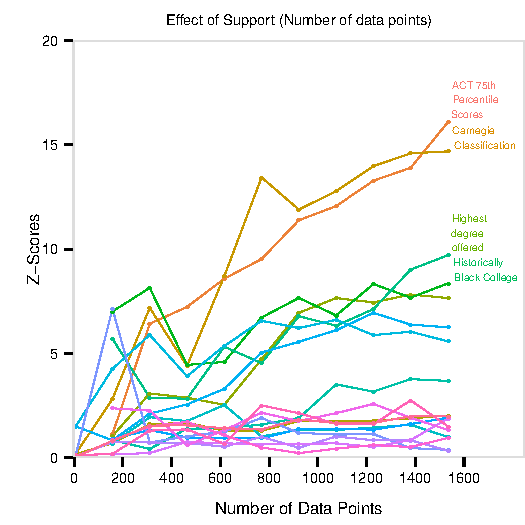
\includegraphics[width=3.25in,height=3.25in]{images/support-nogrid.pdf}
  \caption{The effect of support on the combined z-scores ranking of partitioning variables for the data about US universities. As the number of points in the dataset increase, the importance of the variable determined by the z-scores increases too. }
 \label{fig:support}
\end{figure}
To examine how conservative our approach is in its assessment of good small multiples for those with partitions with low support, we conduct an experiment using the dataset about US universities~\cite{IPEDS}. We compute the rankings based on the combined z-scores for all the partitioning variables in the dataset. Figure~\ref{fig:support} shows these rankings starting with almost all the data points thrown away. Then we progressively add $10\%$ of the data points at random until we recover the full dataset, recomputing the rankings of the partitioning variables at each step. We expect to the see the z-scores generally increasing as the partitions have more points. This confirms the effect of increasing support increasing the importance given to visual patterns by our approach.


\subsection{Parsimonious}
  \begin{figure}
    \centering
    \begin{minipage}[b]{1.7in}
       \begin{subfigure}[b]{\linewidth}
  	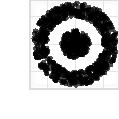
\includegraphics[width=0.75in]{images/donut1-donut2.pdf}
      \caption{}
      \label{fig:pars1}
      \end{subfigure}\\[\baselineskip]
      \begin{subfigure}[b]{\linewidth}
  	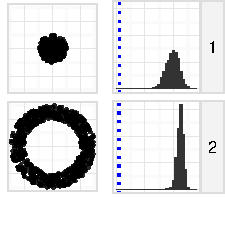
\includegraphics[width=1.65in]{images/19_5065416601259-cluster.pdf}
      \caption{}
      \label{fig:pars2}
      \end{subfigure}
      \begin{subfigure}[b]{\linewidth}
  	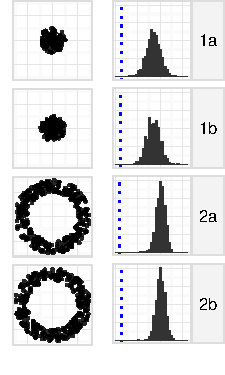
\includegraphics[width=1.65in]{images/9_27395081160431-cluster1.pdf}
        \caption{}
      \label{fig:pars3}        
      \end{subfigure}
    \end{minipage}
    \begin{subfigure}[b]{1.7in}
	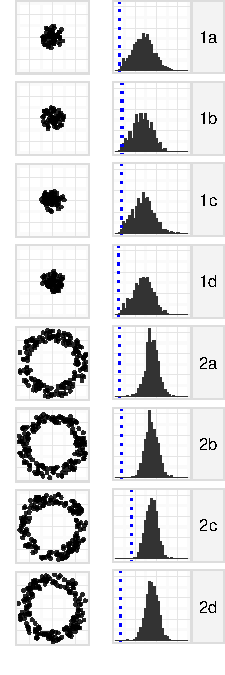
\includegraphics[width=1.7in]{images/5_12851615653375-cluster2.pdf}
      \caption{}
      \label{fig:pars4}
    \end{subfigure}
    \caption{The ranking of small multiple displays respects the parsimony criterion. (a) The original bullseye pattern. (b) The best small multiple determined by the Clumpy scagnostic. (c) The second best partitioning variable redundantly halves the two partitions from (b). (d) The lowest ranked small multiple display with eight partitions.}
    \label{fig:parsimonious}
  \end{figure}

High-cardinality partitioning variables create a large number splits, which likely produce splits with low support as the observations get distributed among more partitions. We want such small multiples to be 
rejected in favor of ones with similar properties except for having fewer partitions. Our algorithm favors small multiples with fewer partitions because of its use of the z-score. (ACTUALLY...I'm not convinced it actually considers the number of partitions explicitly...)

We illustrate the ability of our method to favor parsimonious small multiples using an artificially generated dataset so we can hold the visual patterns across partitioning variables equal as far as possible. We take the bullseye pattern shown in Figure~\ref{fig:pars1} and have a partitioning variable that cleanly separates the ring from the core as seen in Figure~\ref{fig:pars2}. Then we create partitioning variables that repeatedly randomly halve the points in the partitions from the previous step to create small multiples as seen in Figures~\ref{fig:pars3} and~\ref{fig:pars4}. We compute the ranking of these partitioning variables and see the small multiples in the order as shown in Figure~\ref{fig:parsimonious} - top to bottom, left to right. We favor the parsimonious small multiple over the redundant ones that show similar visual patterns with low support. 

